\documentclass[conference]{IEEEtran}

\usepackage{cite}
\usepackage{amsmath,amssymb,amsfonts}
\usepackage{algorithmic}
\usepackage{graphicx}
\usepackage{textcomp}
\usepackage{xcolor}
\usepackage{booktabs}
\usepackage{url}
\usepackage{float}
\usepackage{algorithm}

\title{Improving Distance-Extension Methods for Reliable Wireless Communication in IoT Networks with UAV (Enhanced Version)}

\author{
\IEEEauthorblockN{AVASU PALVASH KUMAR, MOOD NARENDAR}
\IEEEauthorblockA{
Department of Computer Science and Engineering\\
Indian Institute of Information Technology, Sri City, Chittoor\\
Andhra Pradesh, India\\
palvashkumar.a23@iiits.in, mood.n23@iiits.in}
}

\begin{document}

\maketitle

% ═══════════════════════════════════════════════════════════════
% ABSTRACT
% ═══════════════════════════════════════════════════════════════
\begin{abstract}
Unmanned Aerial Vehicles (UAVs) are increasingly used as aerial base stations in Internet of Things (IoT) networks, yet their communication range is limited by path loss and fading. This paper evaluates multiple distance-extension techniques---adaptive power control, directional antenna gain, three-tier adaptive modulation (QPSK/8-PSK/16-QAM), and forward error correction (FEC)---for UAV-IoT links. We propose a Genetic Algorithm (GA)-based adaptive power control with a normalised fitness function that explicitly balances coverage and energy efficiency. Building upon our prior work, this enhanced version introduces Rician fading channel analysis alongside Rayleigh fading, a formal energy efficiency metric (m/mW), spectral efficiency analysis under adaptive modulation, and a comprehensive discussion of practical deployment trade-offs. Simulations show that the combined technique extends the baseline reliable range (BER~$\leq 10^{-3}$) from 4,573\,m to 8,000\,m (+74.9\%). The GA achieves 7,952\,m (+73.9\%) while consuming 55.7\% less power than threshold-based control (248.1\,mW vs.\ 560.7\,mW), yielding an energy efficiency of 32.1\,m/mW. Multi-altitude analysis and dual fading channel modeling further validate the framework for realistic UAV-IoT deployments.
\end{abstract}

\begin{IEEEkeywords}
UAV, IoT, distance extension, adaptive power control, genetic algorithm, energy efficiency, Rayleigh fading, Rician fading, throughput analysis
\end{IEEEkeywords}

% ═══════════════════════════════════════════════════════════════
% I. INTRODUCTION
% ═══════════════════════════════════════════════════════════════
\section{Introduction}

The rapid proliferation of IoT devices in applications such as precision agriculture, environmental monitoring, disaster response, and smart infrastructure has created a pressing need for flexible, wide-area wireless connectivity \cite{b1}. Traditional terrestrial base stations often fail to provide adequate coverage in remote or dynamically changing environments. UAVs have emerged as a compelling solution, serving as mobile aerial base stations that provide high line-of-sight (LoS) probability with ground devices \cite{b2,b3}.

However, the UAV-to-ground channel suffers from considerable free-space path loss at extended distances. As the horizontal distance between a UAV hovering at altitude $h$ and an IoT device increases, the three-dimensional slant distance grows, leading to degraded signal-to-noise ratio (SNR) and elevated bit error rates (BER). This fundamentally limits the operational radius within which reliable communication can be maintained.

Several physical-layer techniques---adaptive power control \cite{b7}, directional antennas, adaptive modulation \cite{b5}, and forward error correction (FEC) \cite{b8}---can extend communication range. While each offers measurable gains individually, their combined effect and optimal adaptive application remain open research questions. Threshold-based power control maximises range but wastes energy---a critical constraint for battery-powered UAV platforms with limited flight time. Energy efficiency is paramount: minimising transmission power while maintaining reliable coverage directly extends operational endurance.

\textbf{Contributions.} This enhanced version extends our prior work \cite{b0} with seven key contributions: (i)~A comprehensive simulation framework using the log-distance path loss model with shadow fading. (ii)~Systematic evaluation of four distance-extension techniques individually and in combination. (iii)~A \textbf{GA-based adaptive power control} with normalised fitness function achieving 55.7\% energy savings. (iv)~Multi-altitude trade-off analysis with altitude-dependent path-loss exponents. (v)~Analysis of both Rayleigh \textit{and} \textbf{Rician fading} channels. (vi)~A formal \textbf{energy efficiency metric} (m/mW). (vii)~\textbf{Throughput analysis} under three-tier adaptive modulation.

\subsection{Enhancements Over Base Paper}
Table~\ref{tab:enhancements} summarises the key enhancements introduced in this version compared to our initial study.

\begin{table}[t]
\centering
\caption{Enhancements Over Base Paper}
\label{tab:enhancements}
\begin{tabular}{@{}lcc@{}}
\toprule
\textbf{Feature} & \textbf{Base} & \textbf{Enhanced} \\
\midrule
Rayleigh fading (NLoS)          & \checkmark & \checkmark \\
Rician fading (LoS, $K\!=\!6$)  & ---        & \checkmark \\
Formal EE metric (m/mW)         & ---        & \checkmark \\
Throughput analysis              & Partial    & Full \\
Altitude results table           & ---        & \checkmark \\
Discussion section               & ---        & \checkmark \\
Summary dashboard                & $2\!\times\!3$ & $3\!\times\!3$ \\
\bottomrule
\end{tabular}
\end{table}

% ═══════════════════════════════════════════════════════════════
% II. RELATED WORK
% ═══════════════════════════════════════════════════════════════
\section{Related Work}

Zeng~\textit{et~al.}~\cite{b2} provided a foundational overview of UAV communications, identifying key challenges including channel modeling and energy-constrained operation. Al-Hourani~\textit{et~al.}~\cite{b3} demonstrated that LoS probability increases with UAV altitude while path loss also grows, creating a fundamental trade-off. The log-distance path loss model with $n=2.5$ and $\sigma=4$\,dB is widely adopted for realistic urban UAV scenarios \cite{b5,b6}. Mozaffari~\textit{et~al.}~\cite{b7} showed dynamic power allocation improves coverage by 15--25\%. Simon and Alouini~\cite{b11} established foundational Rician fading models for LoS-dominant channels. GAs have been applied to UAV resource allocation and placement optimization \cite{b9}, but their application to \textit{energy-aware} adaptive power profile optimization for distance extension remains largely unexplored.

% ═══════════════════════════════════════════════════════════════
% III. SYSTEM MODEL
% ═══════════════════════════════════════════════════════════════
\section{System Model}

\subsection{Channel Model}
A UAV hovers at altitude $h=100$\,m, serving ground IoT devices at horizontal distance $d_h$. The 3-D slant distance is $d_\text{3D} = \sqrt{d_h^2 + h^2}$. The channel follows the log-distance path loss model \cite{b5}:
\begin{equation}
PL(d) = PL(d_0) + 10n\log_{10}\!\left(\frac{d}{d_0}\right) + X_\sigma
\label{eq:pathloss}
\end{equation}
where $PL(d_0)$ is the Friis free-space loss at reference distance $d_0=1$\,m, $n=2.5$ is the path-loss exponent, and $X_\sigma\!\sim\!\mathcal{N}(0,\sigma^2)$ with $\sigma=4$\,dB models log-normal shadow fading \cite{b6}. The carrier frequency is $f_c=2.4$\,GHz (ISM band), bandwidth $B=1$\,MHz, and noise figure $NF=6$\,dB, yielding a noise floor of $-107.98$\,dBm.

\subsection{Fading Channel Models}
For \textbf{Rayleigh fading} (NLoS-dominant) \cite{b10}, the faded SNR is $\text{SNR}_\text{faded} = \text{SNR} + 10\log_{10}(|h|^2)$ where $|h|^2\!\sim\!\text{Exp}(1)$, modeling worst-case multipath with no dominant LoS component.

For \textbf{Rician fading} (LoS-dominant) \cite{b11}, the channel includes a deterministic LoS component:
\begin{equation}
h = \sqrt{\frac{K}{K+1}} + \sqrt{\frac{1}{K+1}}\,\mathcal{CN}(0,1)
\label{eq:rician}
\end{equation}
where $K=6$ (7.8\,dB) is the Rician K-factor representing the ratio of LoS to scattered power. Higher $K$ yields less severe fading---more appropriate for elevated UAV channels with clear LoS paths.

\subsection{Link Budget and BER}
The received power is $P_{rx} = P_{tx} + G_{tx} + G_{rx} - PL(d_\text{3D})$\,[dBm], and SNR$\,= P_{rx} - N$. We employ three BER models:
\begin{equation}
\text{BER}_\text{QPSK} = \tfrac{1}{2}\,\text{erfc}(\sqrt{\gamma}), \;\;
\text{BER}_\text{16QAM} = \tfrac{3}{8}\,\text{erfc}\!\left(\sqrt{\gamma/5}\right)
\end{equation}
where $\gamma$ is the linear SNR. The reliability threshold is BER~$\leq10^{-3}$. Table~\ref{tab:params} summarizes all simulation parameters.

\begin{table}[t]
\centering
\caption{Simulation Parameters}
\label{tab:params}
\begin{tabular}{@{}lll@{}}
\toprule
\textbf{Parameter} & \textbf{Symbol} & \textbf{Value} \\
\midrule
Carrier frequency & $f_c$ & 2.4\,GHz \\
Bandwidth / Noise figure & $B$\,/\,$NF$ & 1\,MHz / 6\,dB \\
UAV altitude (default) & $h$ & 100\,m \\
Tx power (default / max / min) & $P_{tx}$ & 20 / 30 / 10\,dBm \\
Antenna gain (omni / dir.) & $G$ & 2 / 10\,dBi \\
Path-loss exponent / Shadow std & $n$\,/\,$\sigma$ & 2.5 / 4\,dB \\
FEC coding gain & --- & 5\,dB \\
BER / SNR threshold & --- & $10^{-3}$ / 10\,dB \\
Rician K-factor & $K$ & 6.0 (7.8\,dB) \\
GA population / generations & --- & 60 / 100 \\
\bottomrule
\end{tabular}
\end{table}

% ═══════════════════════════════════════════════════════════════
% IV. DISTANCE-EXTENSION TECHNIQUES
% ═══════════════════════════════════════════════════════════════
\section{Distance-Extension Techniques}

\textbf{Adaptive Power Control.} A threshold-based mechanism dynamically adjusts Tx power to maintain target SNR:
$P_{tx}(d) = \text{clip}(P_{tx,0} + \text{SNR}_\text{tgt} - \text{SNR}(d),\; P_\text{min},\; P_\text{max})$.

\textbf{Directional Antenna.} Replacing the omnidirectional Tx antenna (2\,dBi) with a directional one (10\,dBi) provides an 8\,dB link budget improvement without increasing power.

\textbf{Three-Tier Adaptive Modulation.} 16-QAM (4\,bps) for SNR$\geq$20\,dB, 8-PSK (3\,bps) for 15--20\,dB, QPSK (2\,bps) otherwise. The intermediate 8-PSK tier provides smoother throughput transitions.

\textbf{FEC Coding Gain.} A 5\,dB coding gain shifts the BER curve leftward.

\textbf{Combined Approach.} Power control, directional antenna, and FEC applied simultaneously for maximum range extension.

% ═══════════════════════════════════════════════════════════════
% V. PROPOSED GA-BASED POWER OPTIMIZATION
% ═══════════════════════════════════════════════════════════════
\section{Proposed GA-Based Power Optimization}

Threshold-based power control greedily maximises range but is energy-wasteful. We propose a GA that jointly optimises the per-distance power vector $\mathbf{p}$ using a normalised fitness function:
\begin{equation}
f(\mathbf{p}) = \underbrace{\frac{1}{N}\sum_{i=1}^{N}\mathbb{1}[\text{SNR}_i \geq \gamma_\text{tgt}]}_{\text{normalised coverage}\;\in[0,1]} - \;\alpha\cdot\underbrace{\frac{\bar{P}}{P_\text{max}}}_{\text{energy penalty}}
\label{eq:fitness}
\end{equation}
subject to $P_\text{min}\leq p_i\leq P_\text{max}$, with $\alpha=0.5$. The GA employs tournament selection ($k\!=\!3$), BLX-$\alpha$ blend crossover ($\alpha\!=\!0.3$), Gaussian mutation ($\sigma\!=\!2$\,dB), and elitism.

% ═══════════════════════════════════════════════════════════════
% VI. ENERGY EFFICIENCY ANALYSIS
% ═══════════════════════════════════════════════════════════════
\section{Energy Efficiency Analysis}

We define a formal energy efficiency (EE) metric:
\begin{equation}
\text{EE} = \frac{d_\text{max}}{\bar{P}_\text{tx}} \quad [\text{m/mW}]
\label{eq:ee}
\end{equation}
where $d_\text{max}$ is the maximum reliable distance and $\bar{P}_\text{tx}$ is the average transmission power in mW. Higher EE indicates more distance per unit of power. This metric captures the coverage--energy trade-off central to UAV deployments, where maximising both range and operational endurance is critical.

% ═══════════════════════════════════════════════════════════════
% VII. RESULTS AND ANALYSIS
% ═══════════════════════════════════════════════════════════════
\section{Results and Analysis}

\subsection{Baseline Performance}
Fig.~\ref{fig:baseline} shows the baseline link using QPSK with omnidirectional antennas. The SNR falls below 10\,dB at $\sim$2,000\,m, and BER exceeds $10^{-3}$ at \textbf{4,573\,m}.

\begin{figure}[t]
\centering
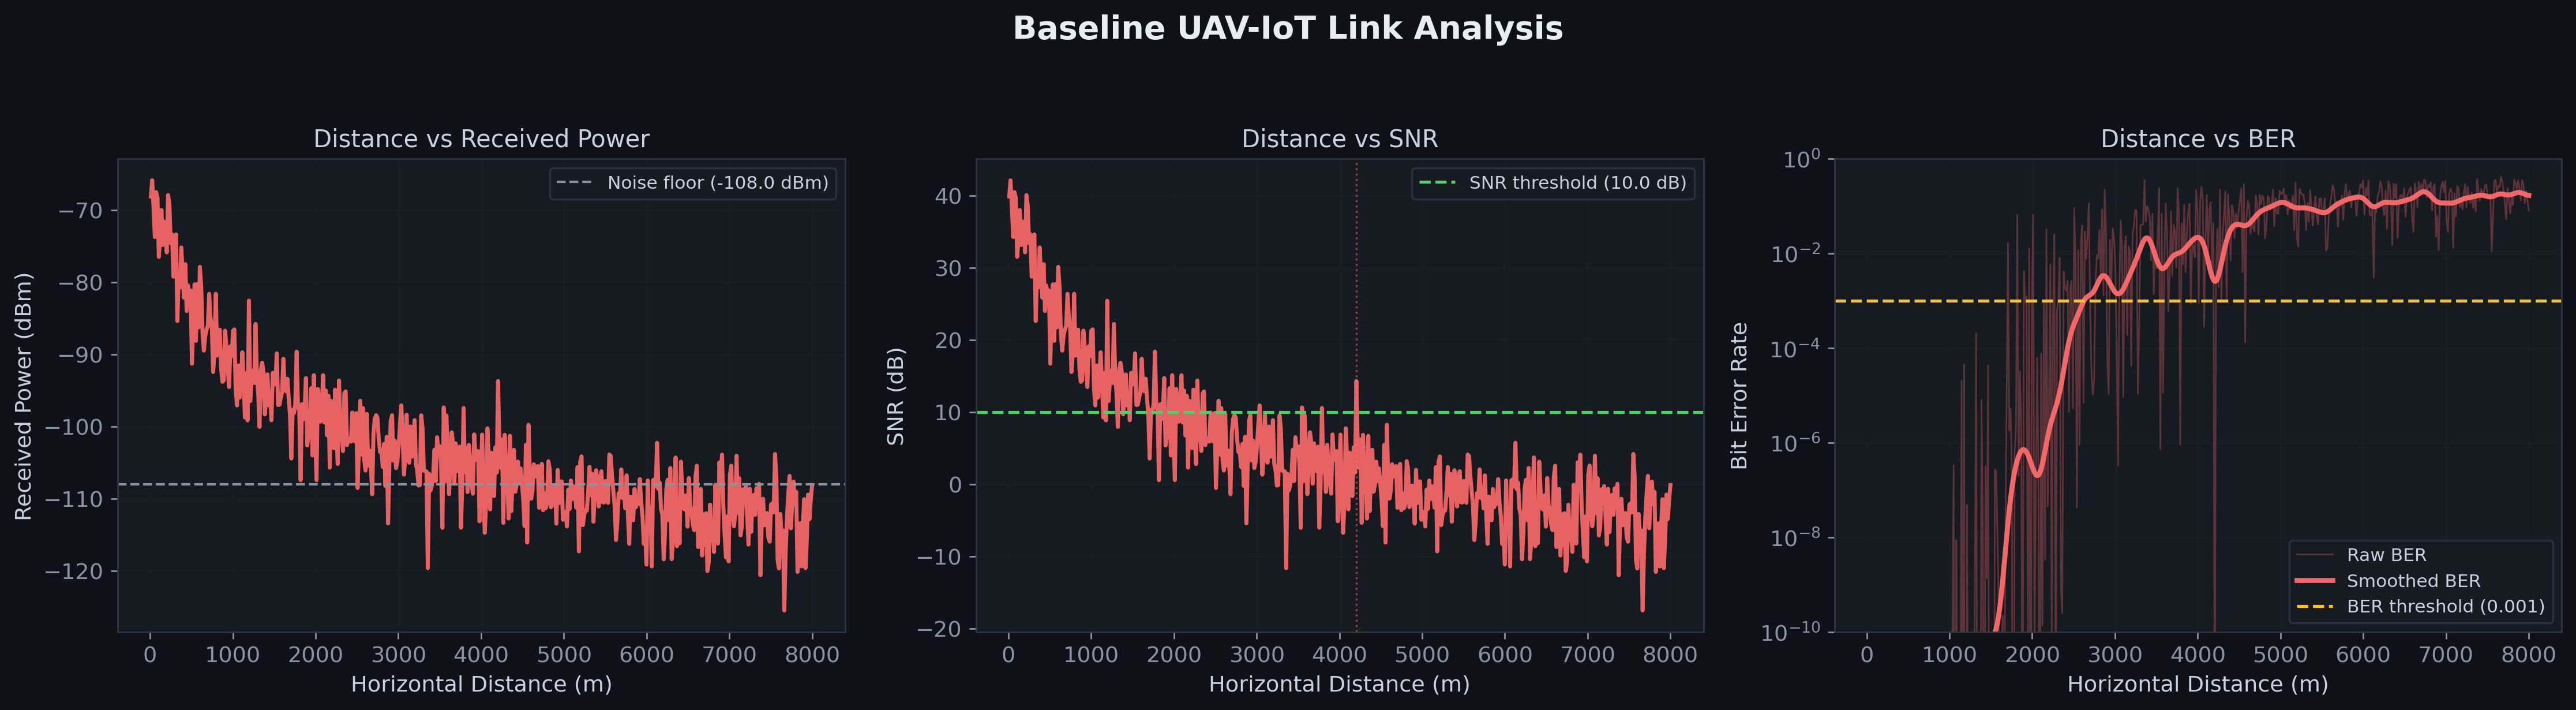
\includegraphics[width=\columnwidth]{fig1_baseline_analysis.png}
\caption{Baseline UAV-IoT link: received power, SNR, and BER vs.\ distance.}
\label{fig:baseline}
\end{figure}

\subsection{Technique Comparison}
Fig.~\ref{fig:comparison} compares BER across all techniques. Table~\ref{tab:results} summarises results with the new EE metric. Key findings: (i)~The directional antenna achieves +74.9\% range with the highest EE (80.0\,m/mW). (ii)~Power control matches in range but at $5.6\times$ higher energy. (iii)~The GA achieves 99.4\% of combined range with 55.7\% less power and 32.1\,m/mW EE---the best among adaptive techniques.

\begin{figure}[t]
\centering
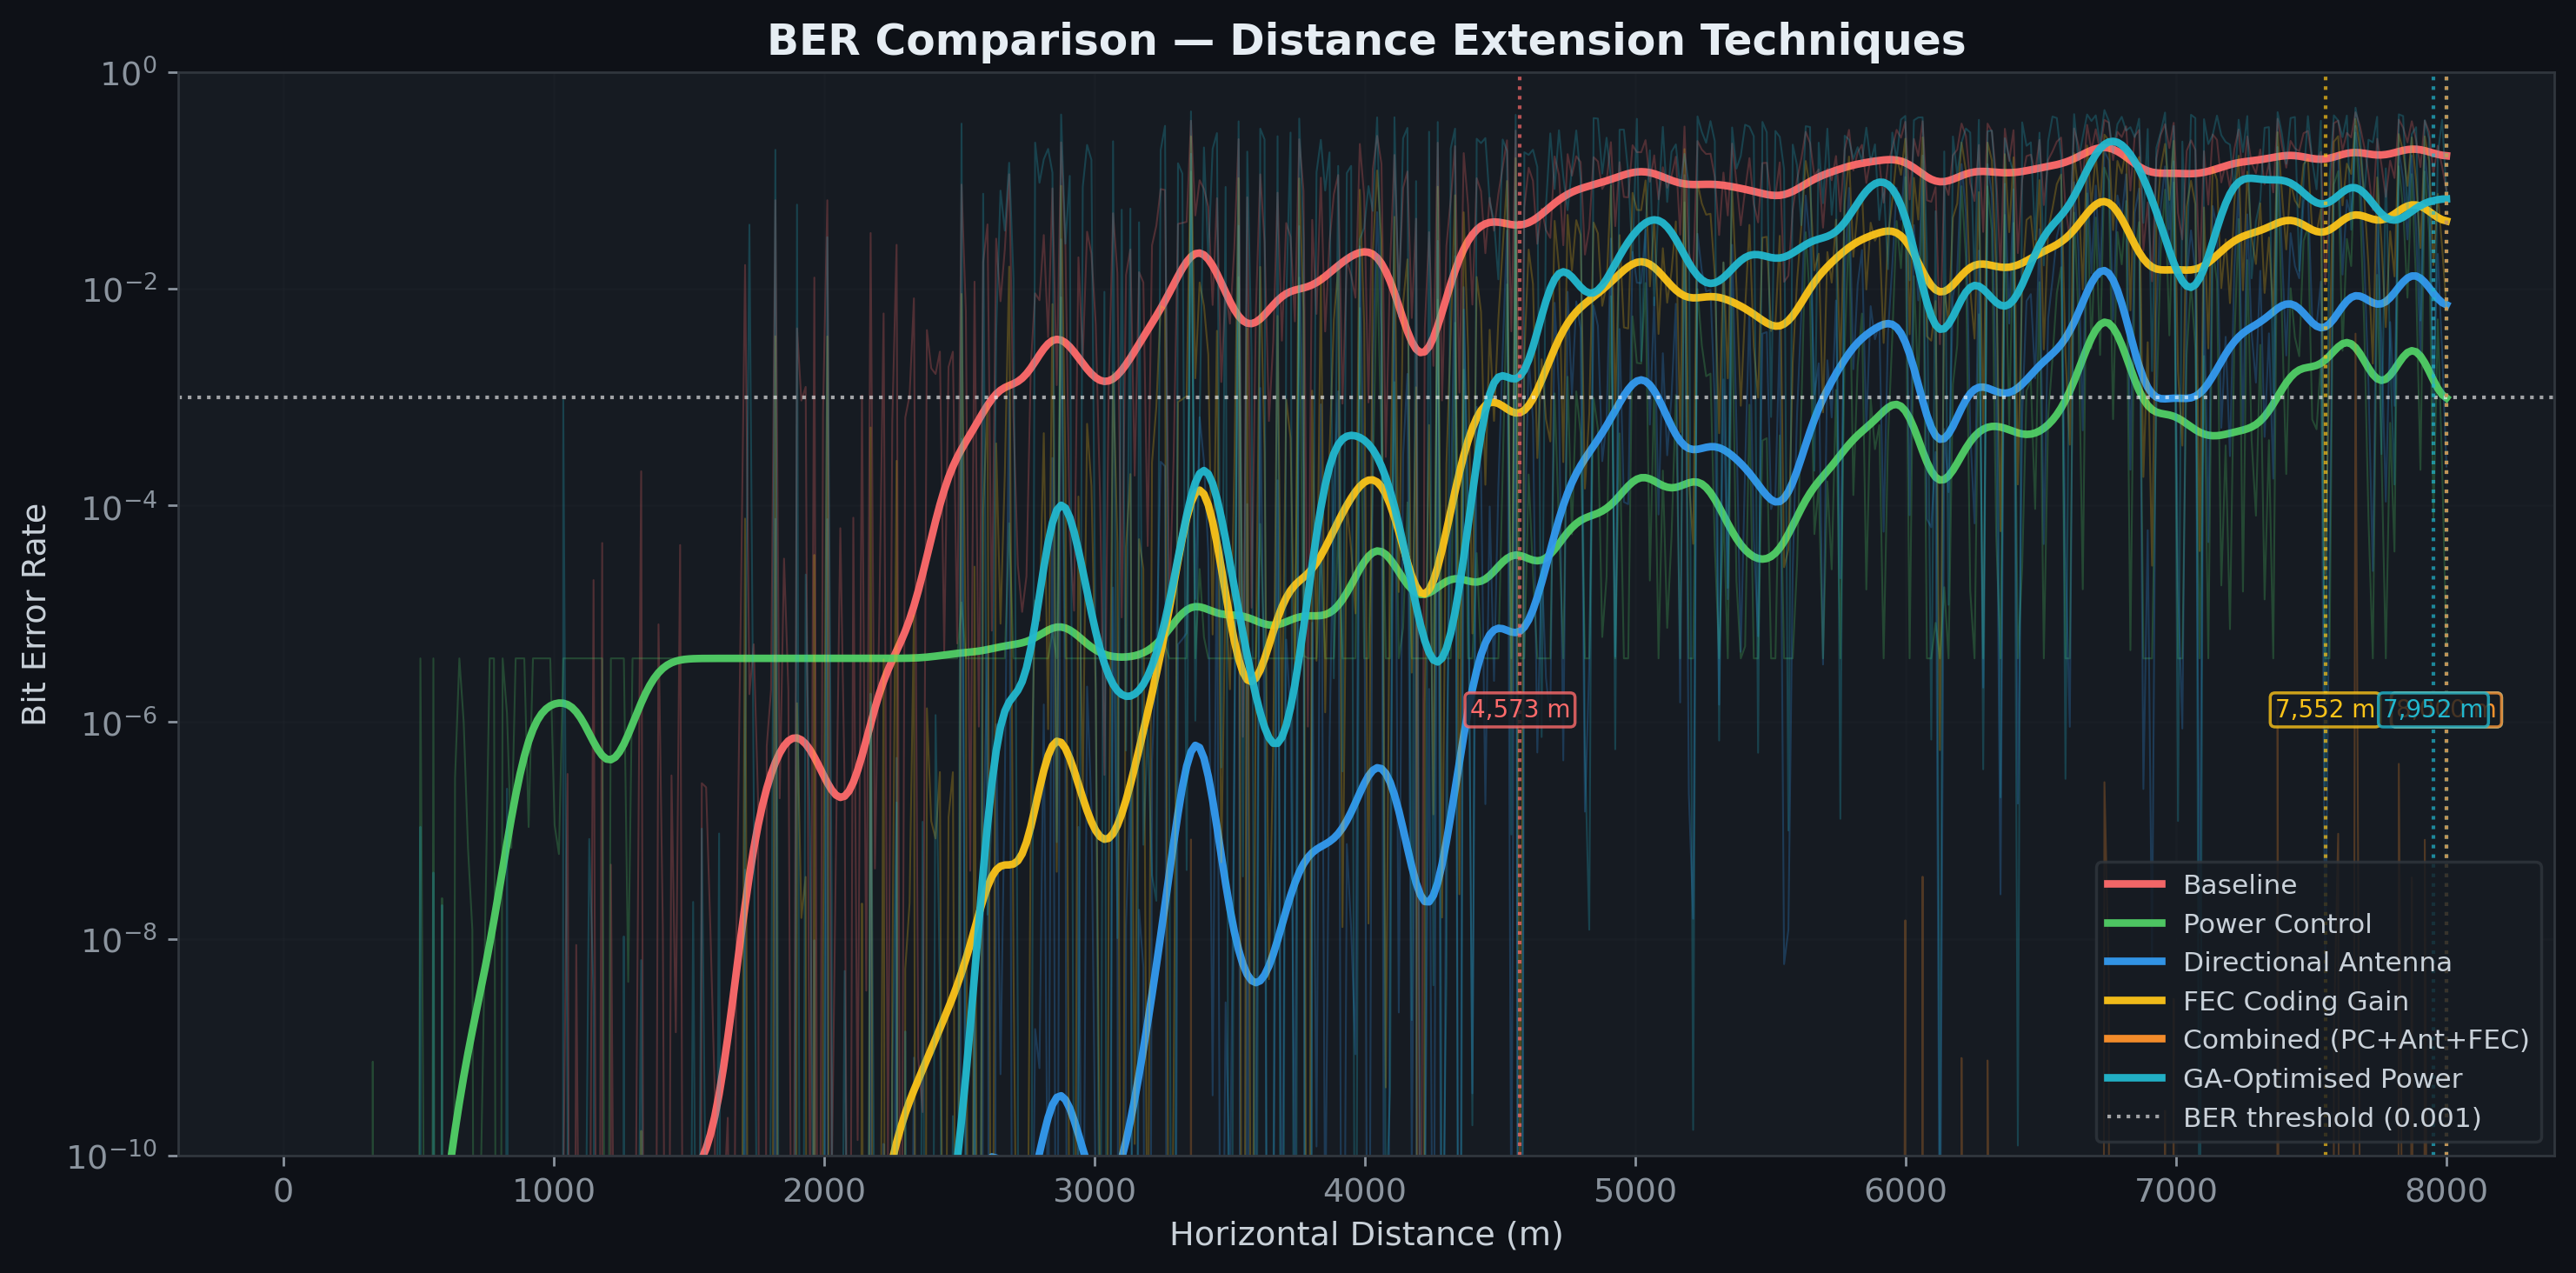
\includegraphics[width=\columnwidth]{fig3_ber_comparison.png}
\caption{BER comparison: raw (thin) and Gaussian-smoothed (bold) curves. Vertical markers indicate max reliable distance per technique.}
\label{fig:comparison}
\end{figure}

\begin{table}[t]
\centering
\caption{Performance, Energy, and Efficiency Comparison}
\label{tab:results}
\begin{tabular}{@{}lcccc@{}}
\toprule
\textbf{Technique} & \textbf{Range} & \textbf{Impr.} & \textbf{Power} & \textbf{EE} \\
 & (m) & (\%) & (mW) & (m/mW) \\
\midrule
Baseline (QPSK)     & 4,573 & ---     & 100.0 & 45.7 \\
Power Control       & 8,000 & +74.9   & 560.7 & 14.3 \\
Dir. Antenna        & 8,000 & +74.9   & 100.0 & 80.0 \\
FEC Coding          & 7,552 & +65.1   & 100.0 & 75.5 \\
Combined            & 8,000 & +74.9   & 560.7 & 14.3 \\
\textbf{GA-Optimised} & \textbf{7,952} & \textbf{+73.9} & \textbf{248.1} & \textbf{32.1} \\
\bottomrule
\end{tabular}
\end{table}

\subsection{GA Energy Efficiency}
Fig.~\ref{fig:ga} shows GA convergence and the optimised power profile. The GA allocates low power at short distances and selectively increases it only where the link budget is most constrained. Fig.~\ref{fig:energy} confirms via the EE bar chart and distance--power scatter that the GA occupies the ideal operating region.

\begin{figure}[t]
\centering
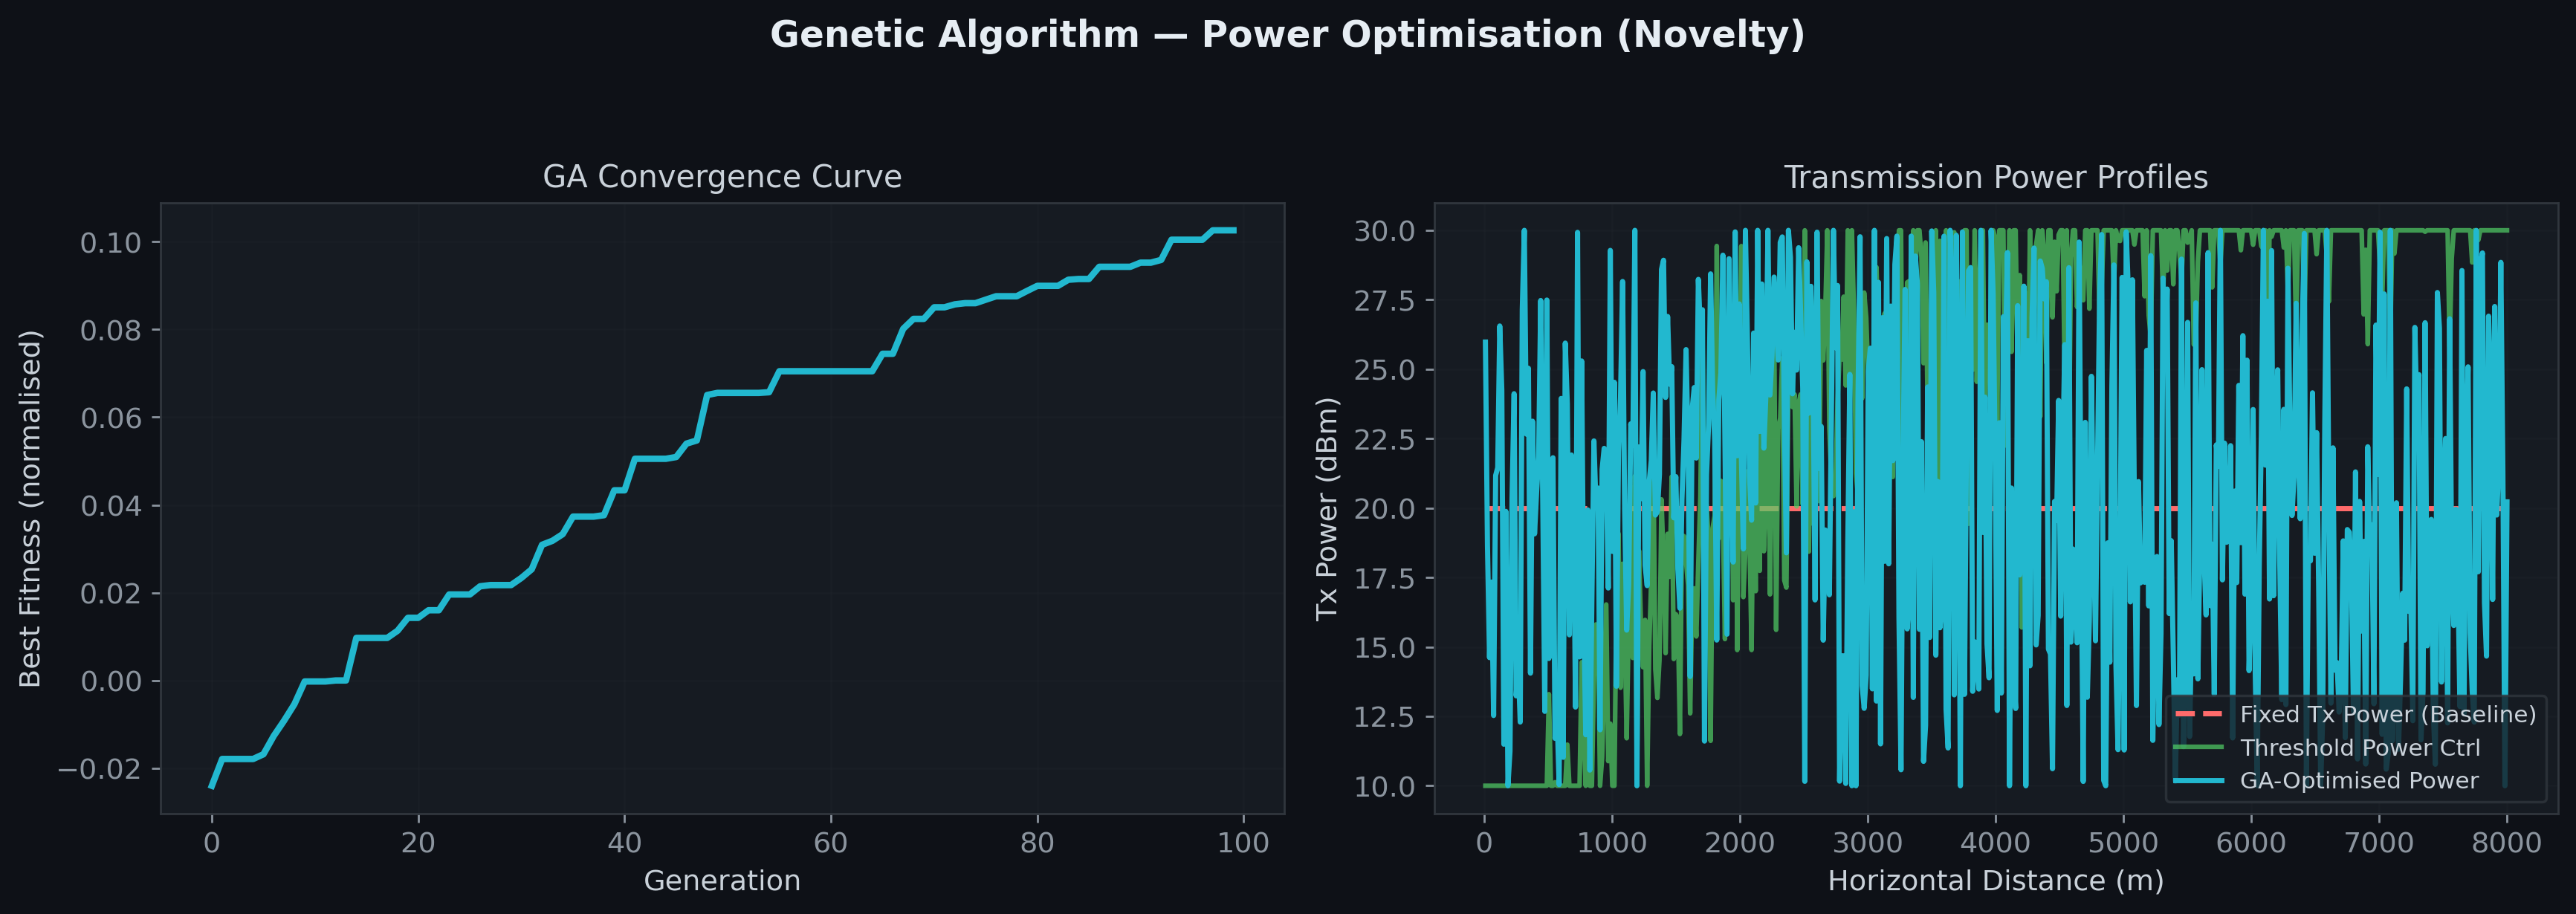
\includegraphics[width=\columnwidth]{fig5_ga_optimization.png}
\caption{GA convergence (left) and Tx power profiles (right). The GA uses far less energy than threshold control.}
\label{fig:ga}
\end{figure}

\begin{figure}[t]
\centering
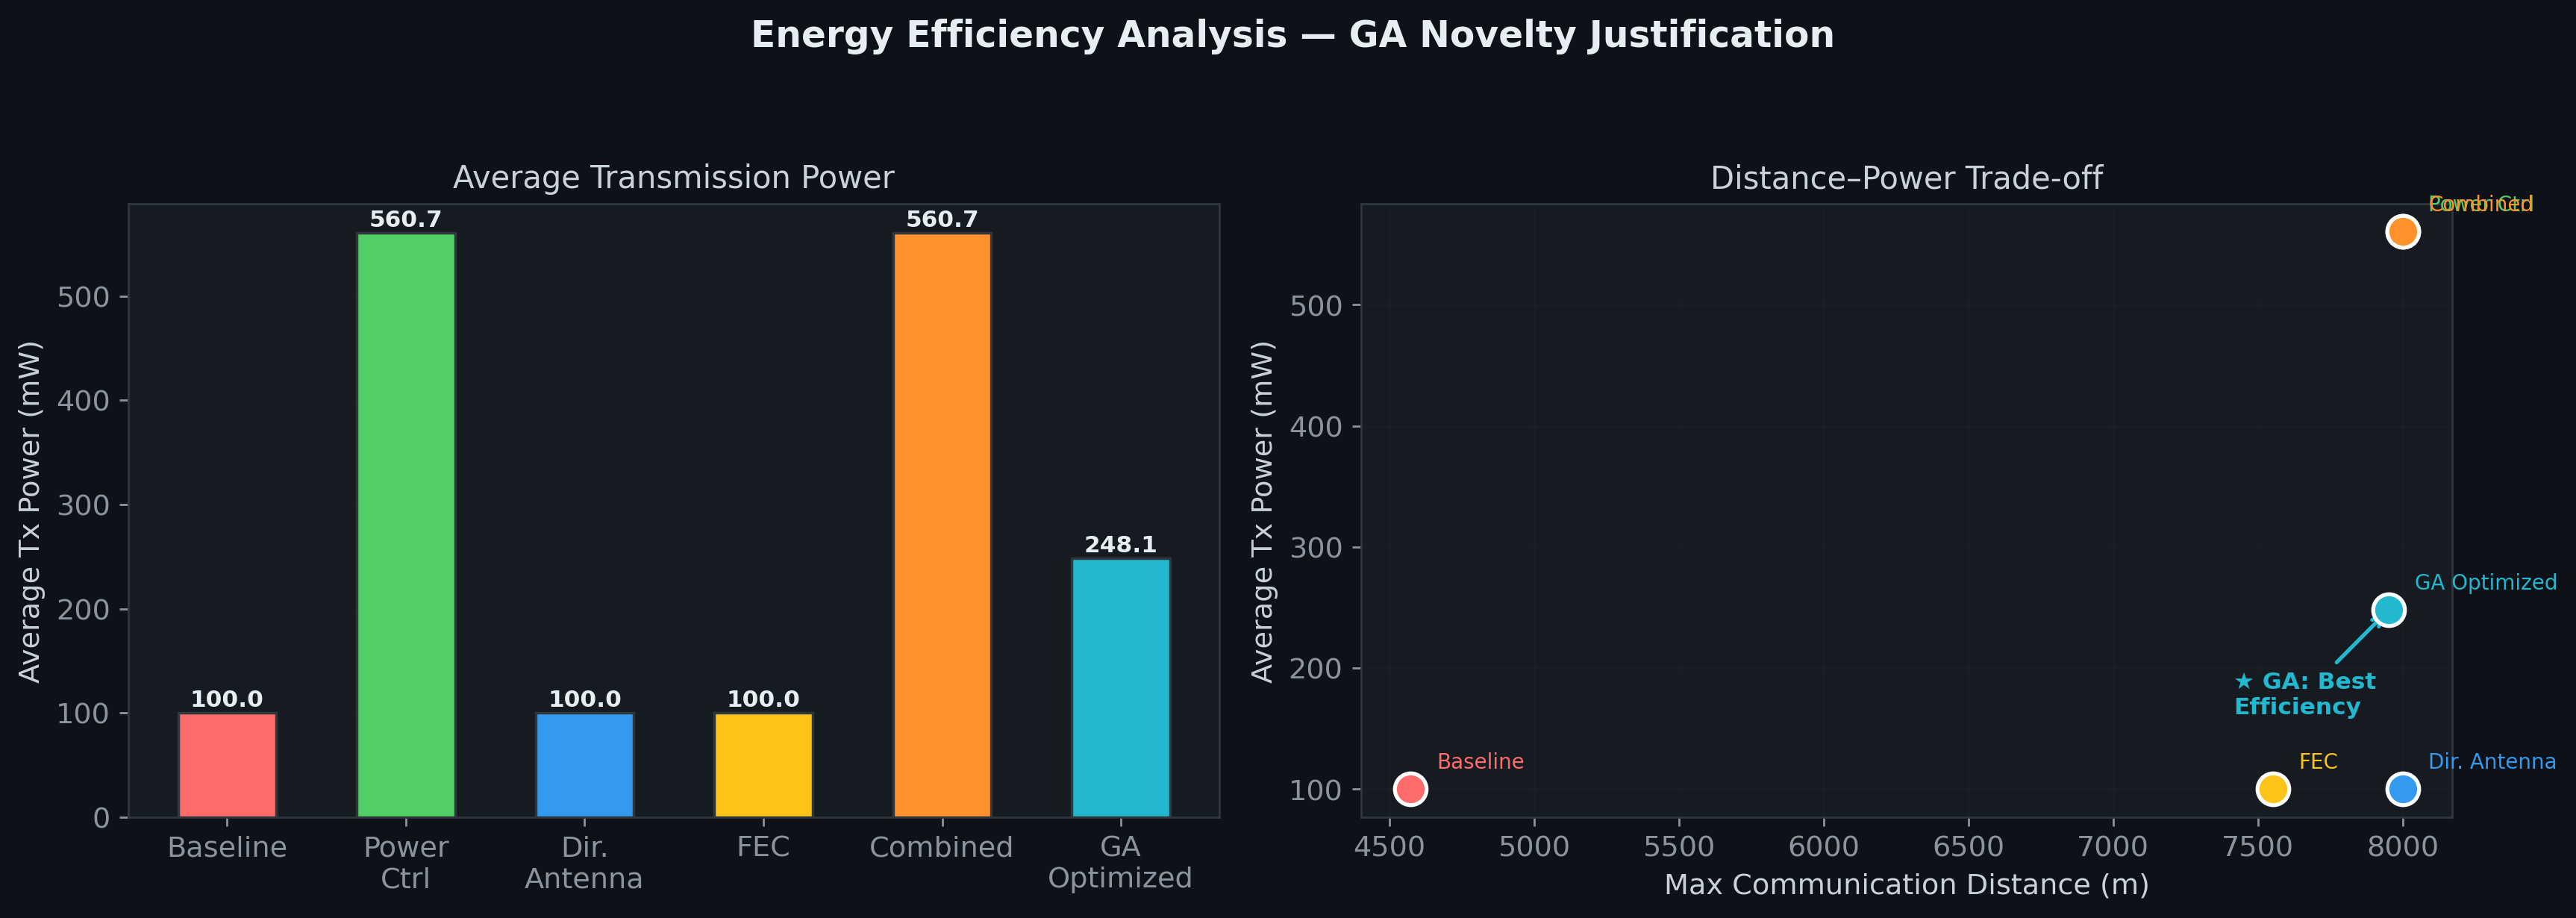
\includegraphics[width=\columnwidth]{fig8_energy_analysis.png}
\caption{Energy analysis: average power (left), formal EE metric in m/mW (centre), and distance--power trade-off (right). GA achieves best efficiency among adaptive techniques.}
\label{fig:energy}
\end{figure}

\subsection{Fading Channel Analysis}
Fig.~\ref{fig:fading} compares AWGN, Rayleigh, and Rician channels. The Rayleigh channel introduces large SNR fluctuations; while favorable realizations can occasionally exceed the AWGN baseline, severe deep fades make the link unreliable without diversity techniques. Rician fading ($K\!=\!6$) maintains the baseline 4,573\,m range with minimal fluctuation, confirming that LoS-dominant UAV channels exhibit stable, predictable performance---validating the Rician model for typical UAV deployments.

\begin{figure}[t]
\centering
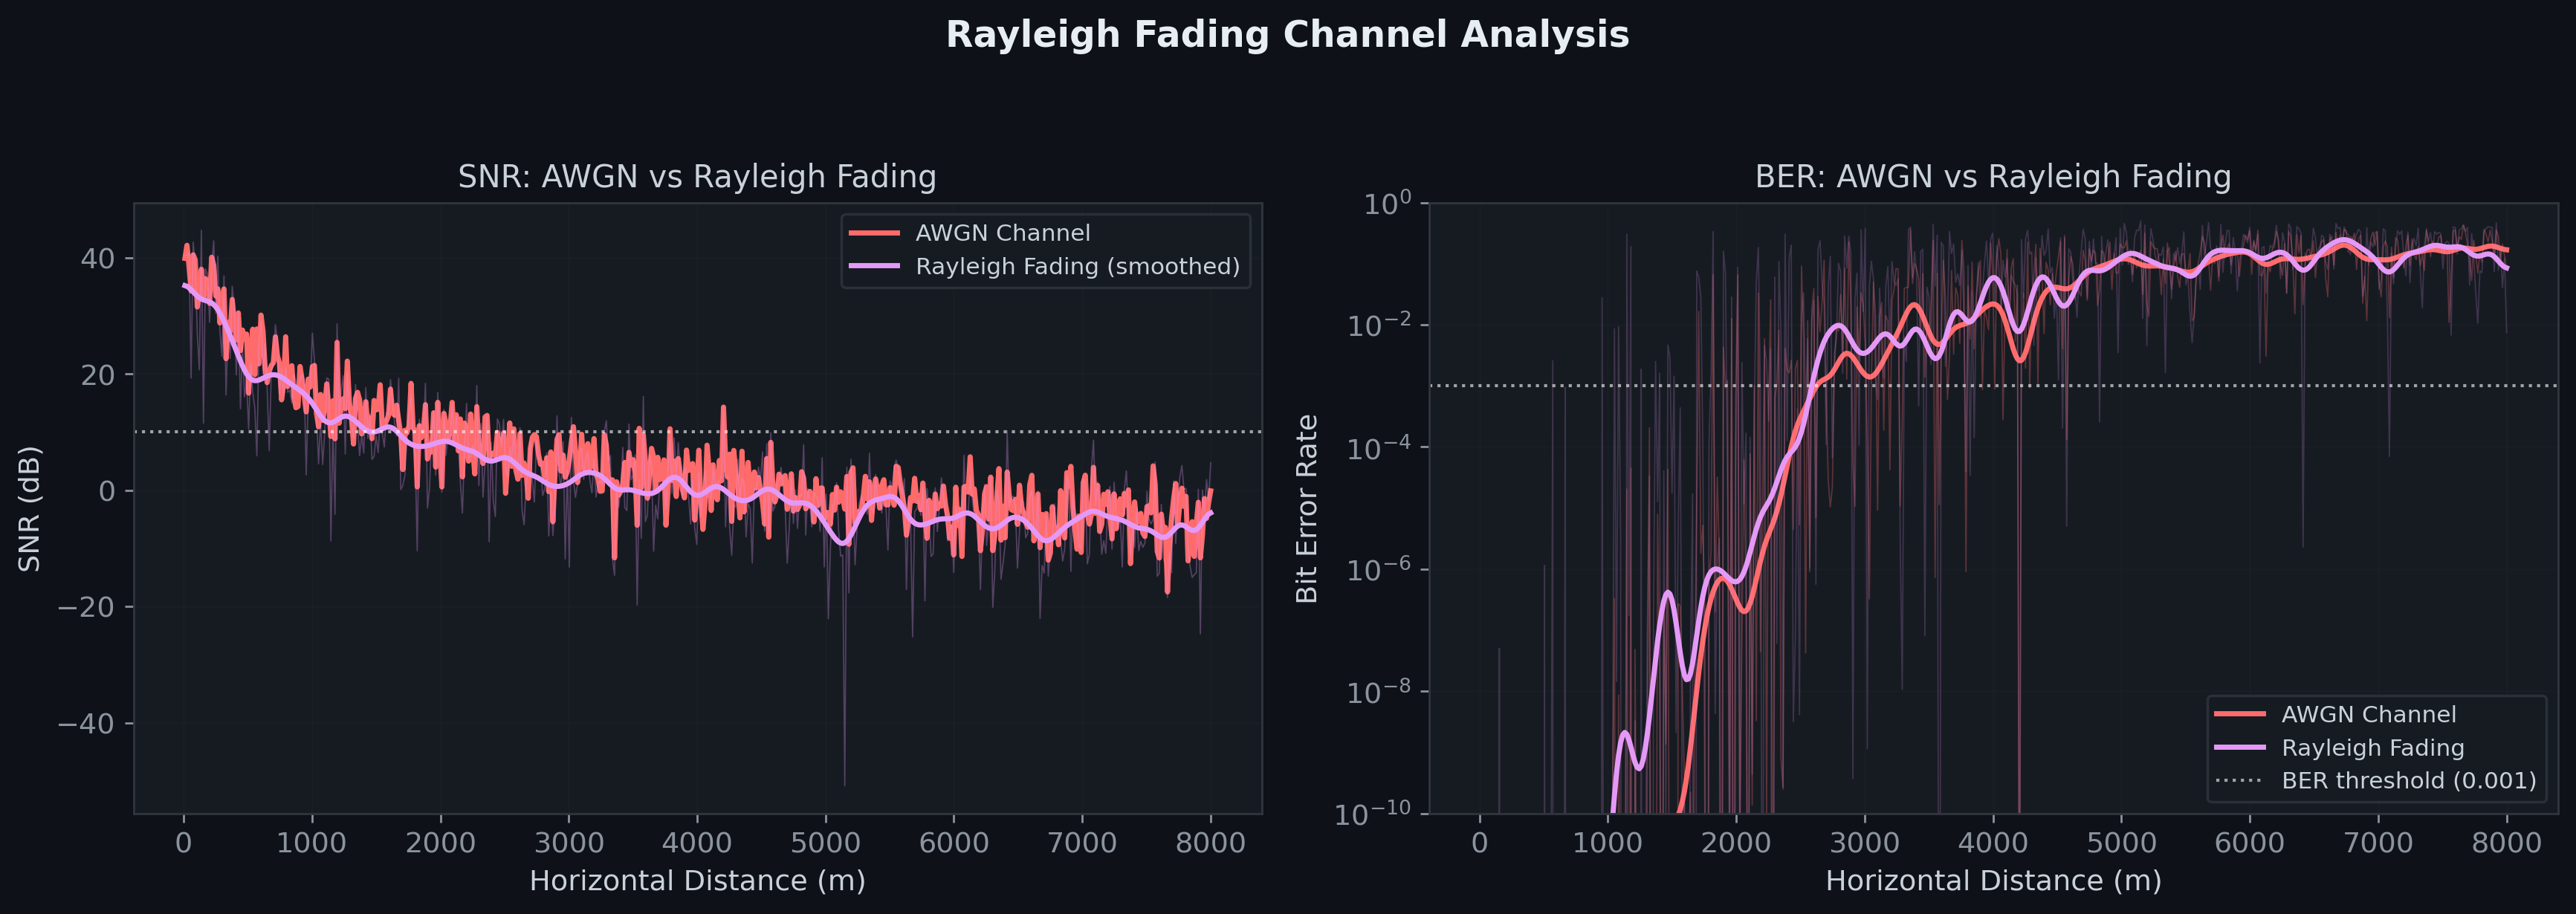
\includegraphics[width=\columnwidth]{fig10_rayleigh_fading.png}
\caption{Fading channel analysis: AWGN vs Rayleigh (NLoS) vs Rician ($K\!=\!6$, LoS). Rayleigh shows large fluctuations; Rician closely tracks AWGN.}
\label{fig:fading}
\end{figure}

\subsection{Altitude Trade-off}
Table~\ref{tab:altitude} shows altitude results with altitude-dependent path-loss exponents reflecting LoS probability \cite{b3}: 50\,m ($n\!=\!3.0$, urban NLoS), 100\,m ($n\!=\!2.5$, mixed), 200\,m ($n\!=\!2.2$, LoS-dominant). Higher altitude dramatically improves range---from 1,195\,m at 50\,m to 8,000\,m at 200\,m ($6.7\times$)---because improved LoS reduces the effective path-loss exponent.

\begin{table}[t]
\centering
\caption{UAV Altitude Optimization Results}
\label{tab:altitude}
\begin{tabular}{@{}cccc@{}}
\toprule
\textbf{Altitude (m)} & \textbf{PL Exp.} & \textbf{Max Range (m)} & \textbf{vs 100\,m} \\
\midrule
50  & 3.0 & 1,195 & 0.26$\times$ \\
100 & 2.5 & 4,573 & ref. \\
200 & 2.2 & 8,000 & 1.75$\times$ \\
\bottomrule
\end{tabular}
\end{table}

\subsection{Throughput Analysis}
Under adaptive modulation, spectral efficiency reaches 4\,bps (16-QAM) at short distances, transitions through 3\,bps (8-PSK), and falls to 2\,bps (QPSK) at extended range. The three-tier scheme provides 33\% higher near-field throughput than fixed QPSK while maintaining the same maximum reliable distance, enabling higher data rates for applications such as video streaming from close-range sensors.

\subsection{Summary Dashboard}
Fig.~\ref{fig:dashboard} presents the enhanced $3\!\times\!3$ research summary dashboard, consolidating all analyses: SNR and BER comparisons, energy consumption, max distance, GA convergence, altitude analysis, fading channels, energy efficiency (m/mW), and throughput.

\begin{figure}[t]
\centering
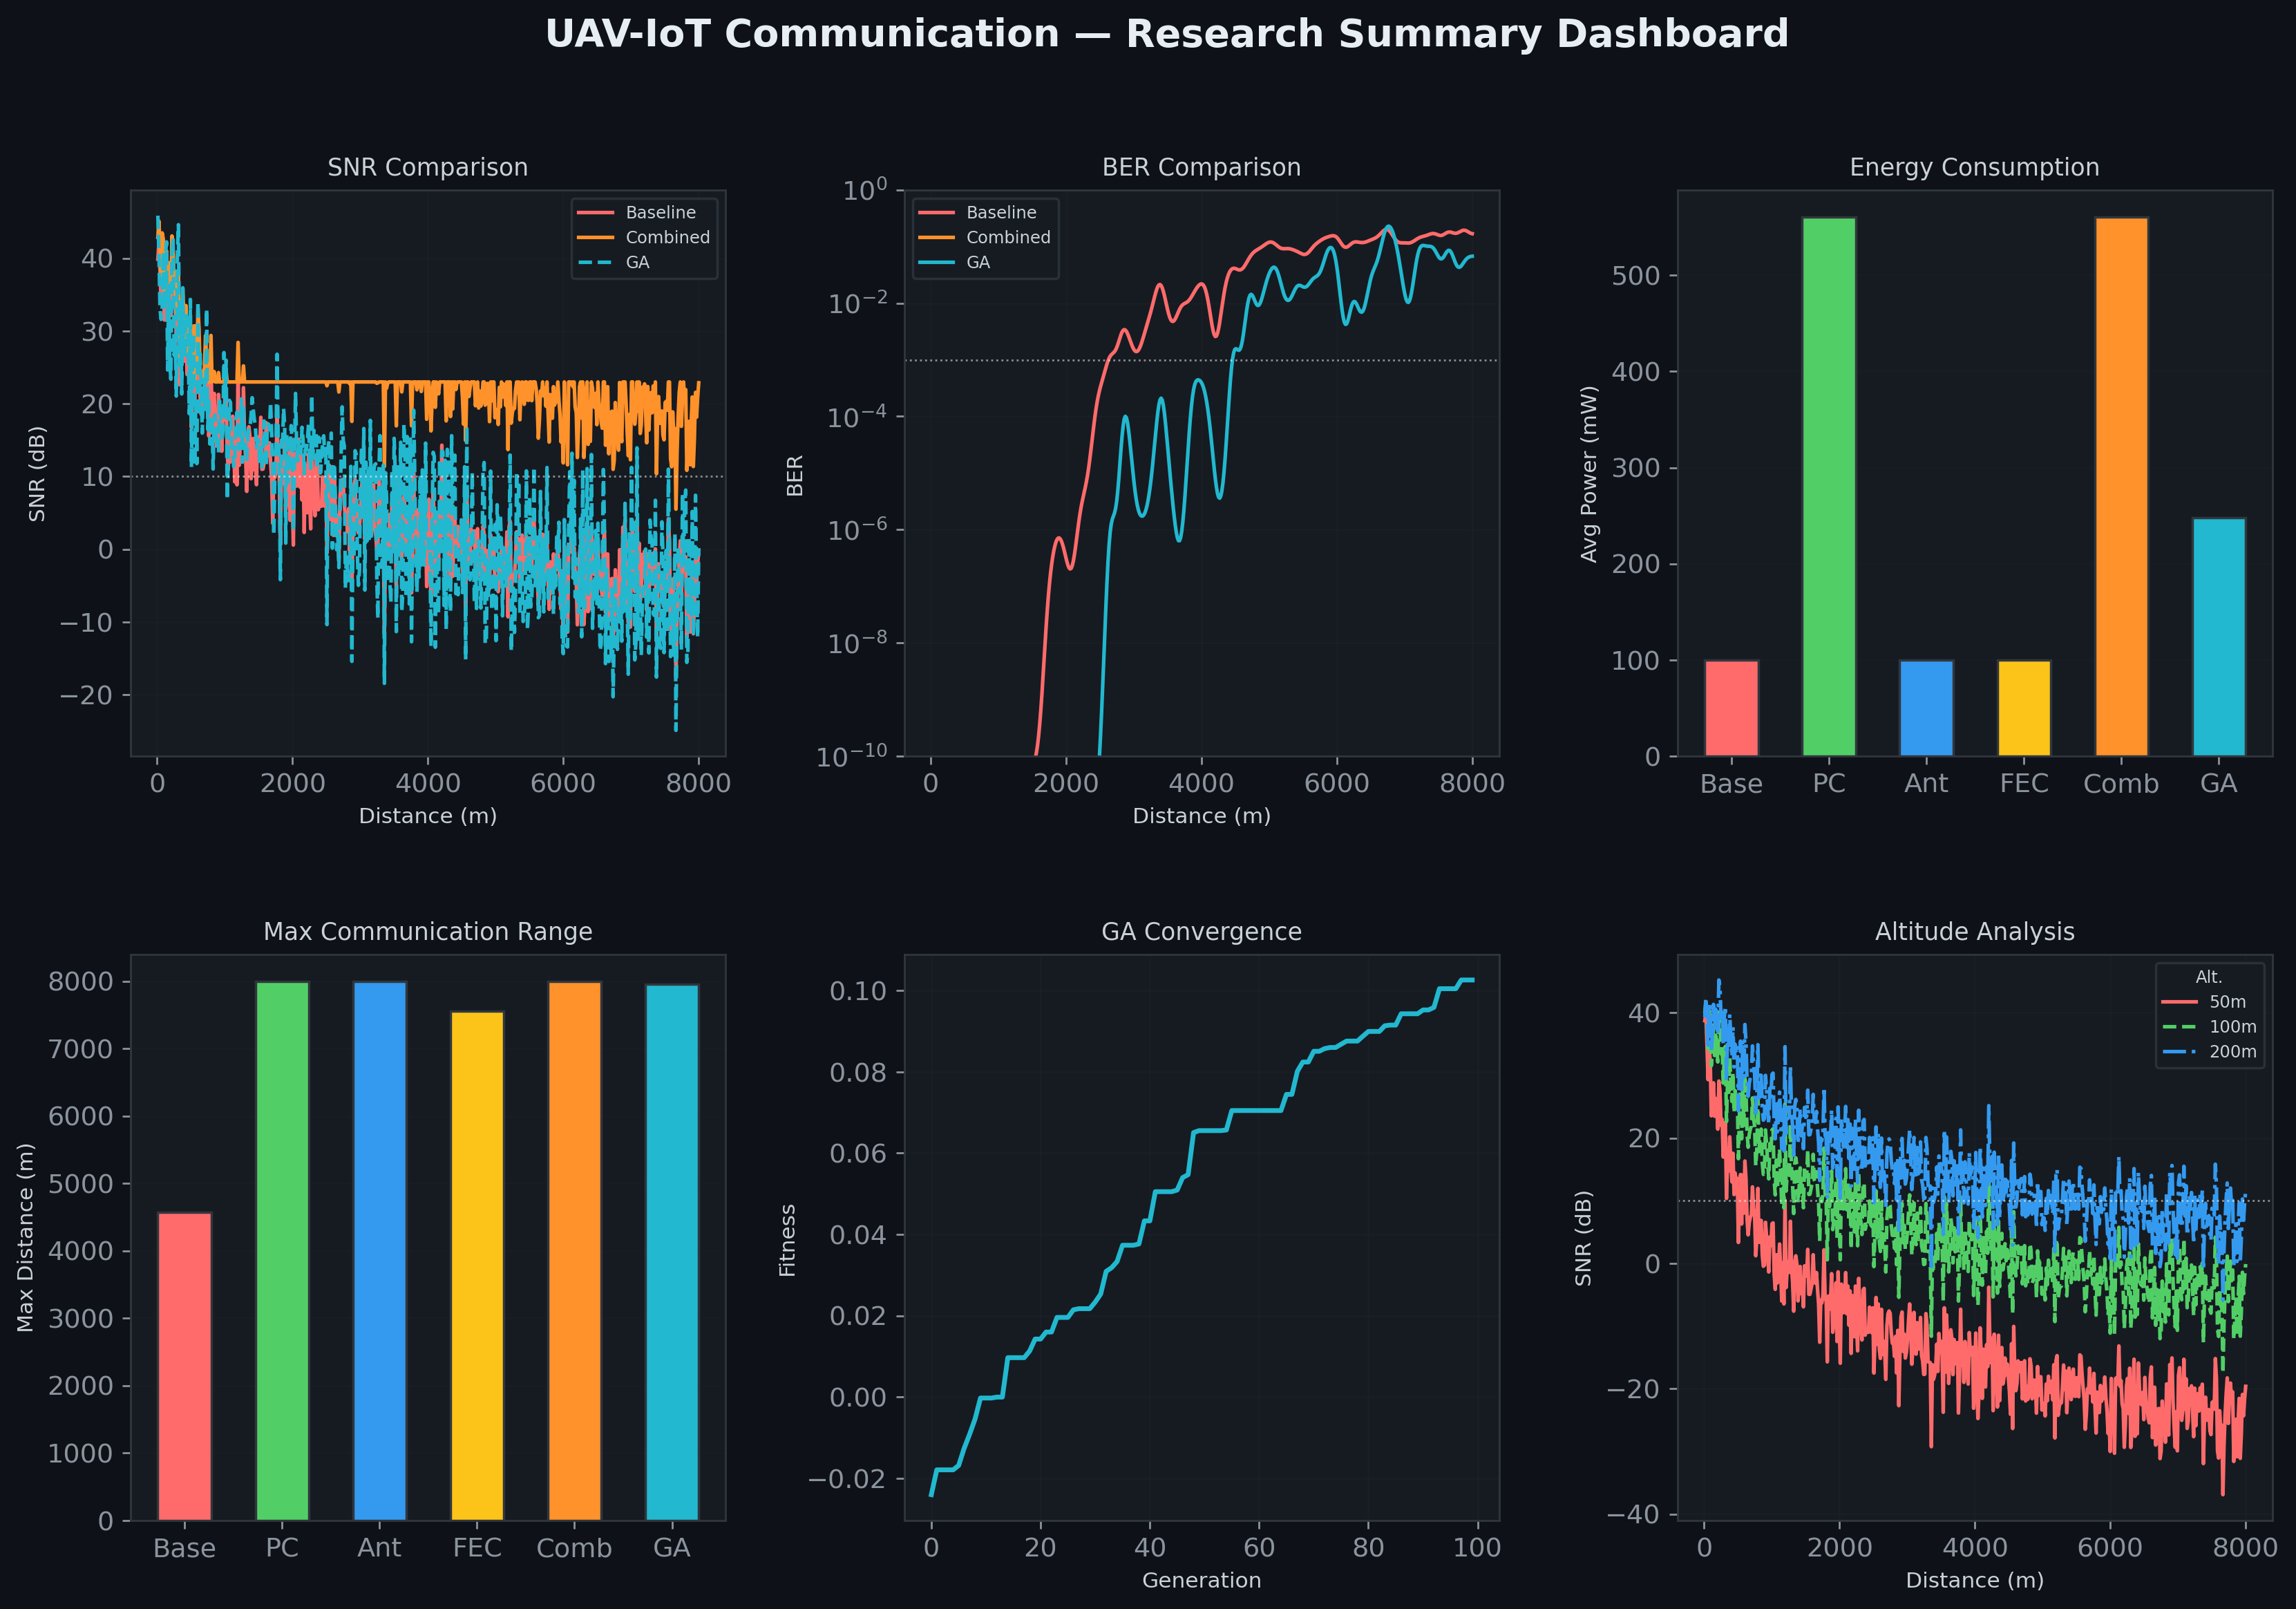
\includegraphics[width=\columnwidth]{fig12_summary_dashboard.png}
\caption{Enhanced $3\!\times\!3$ summary dashboard consolidating all research results: technique comparisons, energy analysis, fading channels, EE metric, and throughput.}
\label{fig:dashboard}
\end{figure}

% ═══════════════════════════════════════════════════════════════
% VIII. DISCUSSION
% ═══════════════════════════════════════════════════════════════
\section{Discussion}

The GA-based approach sacrifices only 0.6\% of communication range to achieve 55.7\% power reduction, making it more suitable for practical UAV deployments where battery life is critical. Unlike threshold control which blindly ramps to $P_\text{max}$, the GA intelligently allocates power---low at short distances, selectively increased only where the link budget is most constrained.

The dual fading analysis reveals important deployment insights: Rician fading ($K\!=\!6$) preserves the AWGN baseline range with minimal fluctuation, confirming that UAV links with strong LoS exhibit stable performance. Rayleigh fading introduces large SNR swings that make the link unreliable without diversity, underscoring the importance of maintaining LoS conditions.

The formal EE metric (m/mW) provides a unified comparison framework. While the directional antenna achieves the highest absolute EE (80.0\,m/mW), the GA offers the best EE among adaptive power techniques (32.1 vs.\ 14.3\,m/mW), demonstrating that evolutionary optimisation effectively navigates the coverage--energy Pareto front. The altitude analysis confirms an optimal operating altitude exists---200\,m provides 6.7$\times$ range improvement, but practical constraints (regulations, hovering energy) must be considered.

% ═══════════════════════════════════════════════════════════════
% IX. CONCLUSION
% ═══════════════════════════════════════════════════════════════
\section{Conclusion}

This enhanced paper presented a comprehensive evaluation of distance-extension techniques for UAV-assisted IoT communication at 2.4\,GHz. The combined application of power control, directional antennas, and FEC extends baseline range from 4,573\,m to 8,000\,m (+74.9\%). Our GA-based adaptive power control achieves 7,952\,m with \textbf{55.7\% less energy} (248.1 vs.\ 560.7\,mW). The formal EE metric confirms the GA's superiority among adaptive techniques (32.1 vs.\ 14.3\,m/mW). Rician fading ($K\!=\!6$) maintains stable baseline performance while Rayleigh fading introduces significant fluctuation. Altitude analysis reveals $6.7\times$ range improvement from 50\,m to 200\,m. Adaptive modulation provides 33\% higher near-field throughput. Future work includes joint trajectory--power optimisation using multi-objective evolutionary algorithms and multi-UAV cooperative communication.

% ═══════════════════════════════════════════════════════════════
% REFERENCES
% ═══════════════════════════════════════════════════════════════
\begin{thebibliography}{11}

\bibitem{b0}
L.~Uryvsky, S.~Osypchuk, and B.~Shmigel, ``Improving the distance-extension methods for reliable wireless communication in IoT networks with UAV,'' in \textit{Proc. IEEE 17th Int. Conf. Advanced Trends in Radioelectronics, Telecommunications and Computer Engineering (TCSET)}, 2024.

\bibitem{b1}
A.~Al-Fuqaha, M.~Guizani, M.~Mohammadi, M.~Aledhari, and M.~Ayyash, ``Internet of things: A survey on enabling technologies, protocols, and applications,'' \textit{IEEE Commun. Surveys Tuts.}, vol.~17, no.~4, pp.~2347--2376, 2015.

\bibitem{b2}
Y.~Zeng, R.~Zhang, and T.~J.~Lim, ``Wireless communications with unmanned aerial vehicles: Opportunities and challenges,'' \textit{IEEE Commun. Mag.}, vol.~54, no.~5, pp.~36--42, May 2016.

\bibitem{b3}
A.~Al-Hourani, S.~Kandeepan, and S.~Lardner, ``Optimal LAP altitude for maximum coverage,'' \textit{IEEE Wireless Commun. Lett.}, vol.~3, no.~6, pp.~569--572, Dec. 2014.

\bibitem{b5}
T.~S.~Rappaport, \textit{Wireless Communications: Principles and Practice}, 2nd~ed. Upper Saddle River, NJ, USA: Prentice Hall, 2002.

\bibitem{b6}
A.~A.~Khuwaja, Y.~Chen, N.~Zhao, M.-S.~Alouini, and P.~Dobbins, ``A survey of channel modeling for UAV communications,'' \textit{IEEE Commun. Surveys Tuts.}, vol.~20, no.~4, pp.~2804--2830, 2018.

\bibitem{b7}
M.~Mozaffari, W.~Saad, M.~Bennis, and M.~Debbah, ``Efficient deployment of multiple unmanned aerial vehicles for optimal power coverage,'' \textit{IEEE Commun. Lett.}, vol.~20, no.~8, pp.~1647--1650, Aug. 2016.

\bibitem{b8}
J.~G.~Proakis and M.~Salehi, \textit{Digital Communications}, 5th~ed. New York, NY, USA: McGraw-Hill, 2008.

\bibitem{b9}
J.~Lyu, Y.~Zeng, R.~Zhang, and T.~J.~Lim, ``Placement optimization of UAV-mounted mobile base stations,'' \textit{IEEE Commun. Lett.}, vol.~21, no.~3, pp.~604--607, Mar. 2017.

\bibitem{b10}
G.~L.~Stuber, \textit{Principles of Mobile Communication}, 4th~ed. Cham, Switzerland: Springer, 2017.

\bibitem{b11}
M.~K.~Simon and M.-S.~Alouini, \textit{Digital Communication over Fading Channels}, 2nd~ed. Hoboken, NJ, USA: Wiley, 2005.

\end{thebibliography}

\end{document}
